\documentclass[tikz,border=3pt]{standalone}
\usepackage[utf8]{inputenc}
\usepackage[T1]{fontenc}
\usepackage{lmodern}
\renewcommand{\familydefault}{\sfdefault}
\usepackage{sansmath}\sansmath
\usepackage{chemfig}
\usepackage{pgfplots}\pgfplotsset{compat=1.18,/pgf/number format/use comma,/pgf/number format/1000 sep={.}}
\usetikzlibrary{arrows.meta,calc,positioning,decorations.pathmorphing,patterns}
% paleta del sitio
\definecolor{nar}{HTML}{E8680C}\definecolor{narc}{HTML}{FFB35C}\definecolor{hielo}{HTML}{FFF3E8}
\definecolor{tinta}{HTML}{1D1D1F}\definecolor{gris}{HTML}{6E6E73}\definecolor{lila}{HTML}{7C5CF0}
\definecolor{azul}{HTML}{2F6FD6}\definecolor{menta}{HTML}{17A673}\definecolor{coral}{HTML}{E8342A}
\begin{document}
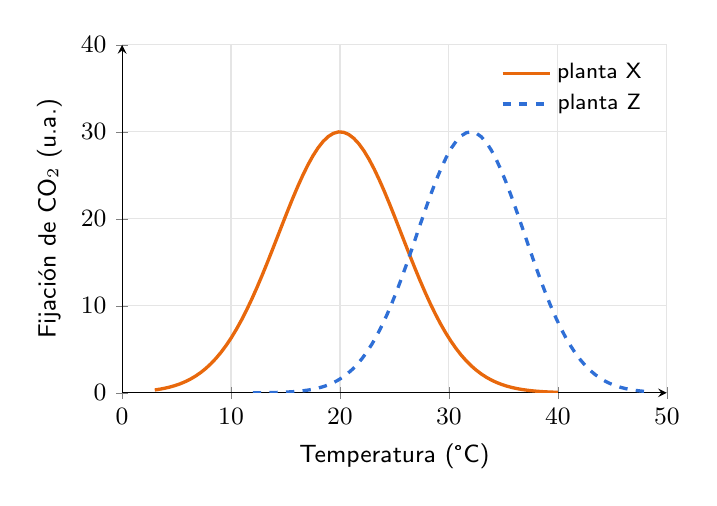
\begin{tikzpicture}[font=\small]
\begin{axis}[width=8.5cm,height=6cm,axis lines=left,xmin=0,xmax=50,ymin=0,ymax=40,xtick={0,10,...,50},ytick={0,10,...,40},xlabel={Temperatura (°C)},ylabel={Fijación de CO$_2$ (u.a.)},grid=major,grid style={gray!20},legend style={draw=none,fill=none,at={(0.98,0.98)},anchor=north east,font=\footnotesize}]
\addplot[nar,very thick,domain=3:40,samples=80] {30*exp(-((x-20)/8)^2)};
\addlegendentry{planta X}
\addplot[azul,very thick,dashed,domain=12:48,samples=80] {30*exp(-((x-32)/7)^2)};
\addlegendentry{planta Z}
\end{axis}
\end{tikzpicture}
\end{document}
